%====================
% BUILD: xelatex cv.tex
%====================
\documentclass[a4paper]{cv}

\usepackage{enumitem}
\usepackage{multicol}

\graphicspath{{image/}}

\begin{document}

%====================
% HEADER
%====================
\header{radovan}{kuka}{Freelance JavaScript Developer \& Web Components Enthusiast}

%====================
% SIDE BLOCK
%====================

\begin{aside}
	% Photo
	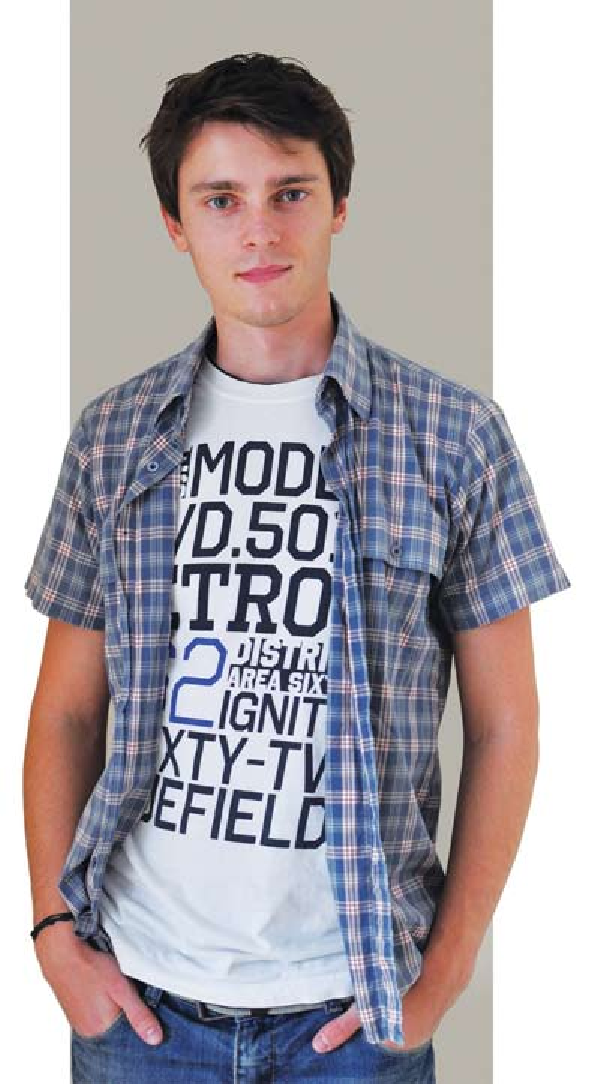
\includegraphics[scale=0.48]{photo.pdf}
	\about{I am a software engineer with strong analytical and logical thinking, highly motivated by challenges and interesting projects. I am a keen learner always seeking to improve my skills and keeping my knowledge up to date.}
	% webpage
	\webpage{www.radovankuka.com}
	% Email
	\email{kuka.radovan@gmail.com}
	% Cellphone
	\phone{(+421) 907 336 220}
	% Address
	\address{Banícka 21}{902 01 Pezinok}{Slovakia}
	% Links
	\section{\vspace{5mm}\linkedIn{http://www.linkedin.com/in/radovankuka}   \github{https://github.com/kuka-radovan}   \twitter{https://twitter.com/radovan_kuka}}
\end{aside}

%====================
% EXPERIENCE
%====================
\section{experience}
\begin{entrylist}
	\entry
		{Full-stack Developer (Freelance)}
		{08/2019 - Present}
		{\emph{Everifin}\\
		I am an coauthor of whole open banking system that aggregates data from european banks through their PSD2 API. We are building universal internet banking application in which users can link all their bank accounts from the EU. They can also send their electronic invoices from our internet banking or pay their bills with one click.}
	\entry
		{Senior Front-End Developer (Freelance)}
		{05/2018 - 08/2019}
		{\emph{Orange Slovensko}\\
		We were implementing e-care system based on microservices and microfrontend architecture. Solution was based on native Web Components (Lit Elements).}
	\entry
		{Senior Front-End Developer (Freelance)}
		{04/2017 - 01/2018}
		{\emph{IN2CORE}\\
		I was hired to kickoff front-end part of cloud based solution of existed software tool for video assist professionals named QTAKE. (React.js, Redux, Babel, Webpack)}
	\entry
		{Front-End Team Lead}
		{06/2016 - 04/2017}
		{\emph{Pygmalios}\\
		I was leading highly motivated front-end team that was developing in-store analytics system - tool dedicated to customer behavior analytics across retail segments. (React.js, Redux, Babel, Webpack)}
	\entry
		{Senior Front-End Developer}
		{04/2015 - 06/2016}
		{\emph{Piano Media}\\
		Front-end developer of paywall system and analytics tool for publishers written in React.js (Redux, Babel, Webpack).}
	...
% 	\entry
% 		{Front-End Team Lead \& Senior Front-End Developer}
% 		{06/2014 - 04/2015}
% 		{\emph{Datalan}\\
% 		I was an author of front-end architecture of modular system for electronic services for city governments written in Ext.js framework.}
% 	\entry
% 		{UI Designer \& Front-End Developer}
% 		{03/2012 - 05/2014}
% 		{\emph{Gratex International}\\
% 		Implementation of custom widgets in Dojo framework and implementation of back office system for international insurance company.}
%	\entry
%		{Java Developer}
%		{12/2010 - 03/2012}
%		{\emph{Vigour}\\
%		Front-end development of a banking system in Finantix framework (Java).}
\end{entrylist}

%====================
% EDUCATION
%====================
\section{education}
\begin{entrylist}
	\entry
		{Slovak University of Technology in Bratislava}
		{2011 - 2013}
		{\emph{Faculty of Informatics and Information Technologies (FIIT)}\\
		Master's degree \emph{(Software Engineering)}}
	\entry
		{Slovak University of Technology in Bratislava}
		{2007 - 2011}
		{\emph{Faculty of Informatics and Information Technologies (FIIT)}\\
		Bachelor's degree \emph{(Informatics)}}
	% \entry
	% 	{Gymnasium of Viliam Pauliny-Tóth in Martin}
	% 	{2003 - 2007}
	% 	{Graduated}
\end{entrylist}

%====================
% CERTIFICATES
%====================
% \section{certificates}
% \begin{entrylist}
% 	\entry
% 		{HTML5 Application Development Fundamentals}
% 		{06/2013}
% 		{\emph{Microsoft Technology Associate (MTA) \\ License: E310-5741}}
% 	\entry
% 		{MongoDB for Developers}
% 		{01/2014}
% 		{\emph{MongoDB, Inc.}}
% \end{entrylist}

%====================
% EXPERTISE
%====================
\section{expertise}
\begin{multicols}{3}

	\centerline{\textbf{Development}}
	\begin{description}[style=multiline,leftmargin=1.8cm,font=\normalfont]
		\item[JavaScript] {\huge\color{red}$\circ\circ\circ\circ\circ$}
		\item[HTML5] {\huge\color{red}$\circ\circ\circ\circ\color{gray}\circ$}
		\item[CSS3] {\huge\color{red}$\circ\circ\circ\color{gray}\circ\circ$}
		%\item[C++] {\huge\color{red}$\circ\circ\circ\color{gray}\circ\circ$}
		%\item[Java] {\huge\color{red}$\circ\circ\circ\color{gray}\circ\circ$}
	\end{description}
	\vfill
	\columnbreak

	\centerline{\textbf{Frameworks \& Tools}}
	\begin{description}[style=multiline,leftmargin=1.8cm,font=\normalfont]
		\item[React] {\huge\color{red}$\circ\circ\circ\circ\color{gray}\circ$}
		\item[Redux] {\huge\color{red}$\circ\circ\circ\circ\color{gray}\circ$}
		%\item[JQuery] {\huge\color{red}$\circ\circ\color{gray}\circ\circ\circ$}
		%\item[OpenCV] {\huge\color{red}$\circ\circ\color{gray}\circ\circ\circ$}
		\item[Vue] {\huge\color{red}$\circ\circ\circ\color{gray}\circ\circ$}
	\end{description}
	\vfill
	\columnbreak

	\centerline{\textbf{Languages}}
	\begin{description}[style=multiline,leftmargin=1.4cm,font=\normalfont]
		\item[Slovak] {\huge\color{red}$\circ\circ\circ\circ\circ$}
		\item[English] {\huge\color{red}$\circ\circ\circ\color{gray}\circ\circ$}
		\item[German] {\huge\color{red}$\circ\color{gray}\circ\circ\circ\circ$}
	\end{description}
	\vfill
	\columnbreak
\end{multicols}

%\section{social skills}
%	communicability, ambitiousness, flexibility, independence, ability to work in a team

\section{interests}
	graphic design, web development, development principles, design patterns, algorithms

%====================
% FOOTER
%====================
\footer{a}{b}{c}
\end{document}
